\chapter{Określenie wymagań oraz projekt graficzny systemu}

\section{Wymagania funkcjonalne}
System ma współpracować z już istniejącym oprogramowaniem Dispatch Rider. W tym celu podjęliśmy się zdefiniowania następujących wymagań funkcjonalnych takich jak:

\begin{enumerate}
	\item Generowanie plików konfiguracyjnych dla Dispatch Ridera:
		\begin{itemize}
			\item generowanie pliku określającego zlecenia, o składni:
			\textbf{ilość-pojazdów ładowność prędkość}
			\item generowanie pliku określającego czas nadchodzenia zleceń, o składni: nr-lini \textbf{czas-zlecenia}
			\item generowanie pliku zawierającego liczbę kierowców
			\item generowanie pliku określającego parametry ciągników, o składni: \textbf{moc niezawodność wygoda zużycie-paliwa typ-zaczepu}
			\item generowanie pliku opisującego parametry naczep o składni: \textbf{masa pojemność typ-ładunku uniwersalność typ-zaczepu}
			\item generowanie pliku opisującego parametry holonów o składni: initialCapacity = \textbf{pojemność-pojazdu} mode = \textbf{tryb} bases = \textbf{ilość-baz} eUnitsCount = \textbf{ilość-jednostek}
			\item generowanie pliku konfiguracyjnego configuration.xml
		\end{itemize}
		
	\item Kolejkowanie zadań zlecanych systemowi.
	
	\item Uruchamianie systemu Dispatch Rider z użyciem dostarczonych z zewnątrz lub wygenerowanych plików konfiguracyjnych
	
	\item Odczyt i parsowanie plików wynikowych Dispatch Ridera, wraz z wizualizacją otrzymanych wyników
		\begin{itemize}
			\item wizualizacja grafu sieci transportowej
			\item wizualizacja tras pokonanych przez pojazdy
			\item wyświetlanie informacji o każdym z holonów 
			\item wyświetlanie zbiorczego podsumowania obliczeń zawierającego koszt, dystans, czas, parametry holonów
		\end{itemize}
	\item Przechowywanie wyników obliczeń, w celu zaprezentowania na żądanie
\end{enumerate}

\section{Wymagania niefunkcjonalne}

\begin{enumerate}
    \item Dokumentacja techniczna w postaci strony wiki, dokumentu tekstowego oraz komentarzy w kodzie programu.
    \item Przenośność - zapewnienie w pełni poprawnego działania programu na najpopularniejszych przeglądarkach oraz systemach operacyjnych.
    \item Płynność działania wizualizacji grafów w oknie przeglądarki.
    \item Łatwość i intuicyjność obsługi, umożliwienie komfortowego korzystania z programu bez poznawania szczegółowych instrukcji dotyczących uruchamiania i konfiguracji.
\end{enumerate}

\section{Przypadki użycia}

Jedynym aktorem w naszym systemie jest Użytkownik - osoba posługująca się systemem za pośrednictwem strony WWW - jest ona w stanie dodawać nowe zadania oraz oglądać wyniki już obliczone.\\

\subsection{Wyświetlenie zadań oczekujących na wykonanie}
	\textbf{Cel przypadku użycia:} Sprawdzenie przez użytkownika jakie zadania zostały już wybrane do wykonania, lecz ich wykonanie się nie rozpoczęło.\\
	\textbf{Aktor:} Użytkownik\\
	\textbf{Warunki początkowe:} Istnieje aplikacja serwera, klient jest do niej podłączony przy pomocy aplikacji klienckiej.\\
	\textbf{Scenariusz:}
	\begin{enumerate}
	\item Użytkownik przełącza się na zakładkę zadań oczekujących
	\item Aplikacja pobiera listę plików znajdujących się w katalogu uploads
	\item  Aplikacja wyświetla listę plików w postaci tabelki\\\\
	\end{enumerate}

\subsection{Wyświetlenie wyników zadań wykonanych}
	\textbf{Cel przypadku użycia:} Sprawdzenie przez użytkownika jakie zadania zostały już wybrane do wykonania, lecz ich wykonanie się nie rozpoczęło.\\
	\textbf{Aktor:} Użytkownik\\
	\textbf{Warunki początkowe:} Istnieje aplikacja serwera, klient jest do niej podłączony przy pomocy aplikacji klienckiej.\\
	\textbf{Scenariusz:}
	\begin{enumerate}
	\item Użytkownik przełącza się na zakładkę zadań oczekujących
	\item Aplikacja pobiera listę plików znajdujących się w katalogu uploads
	\item  Aplikacja wyświetla listę plików w postaci tabelki\\\\
	\end{enumerate}
\subsection{Wizualizacja grafu połączeń}
	\textbf{Cel przypadku użycia:} Przedstawienie użytkownikowi grafu obrazującego sposób poruszania się holonów.\\
	\textbf{Aktor:} Użytkownik\\
	\textbf{Warunki początkowe:} Istnieje aplikacja serwera, klient jest do niej podłączony przy pomocy aplikacji klienckiej. Dany zestaw został obliczony\\
	\textbf{Scenariusz:}
	\begin{enumerate}
	\item Użytkownik przełącza się na zakładkę zadań obliczonych
	\item Aplikacja pobiera listę plików znajdujących się w katalogu ready i wyświetla je
	\item Użytkownik klika na wybrany model obliczeń
	\item Aplikacja wyświetla graf ukazujący trasy holonów\\\\
	\end{enumerate}
	
\subsection{Generowanie pliku określającego zlecenia}
	\textbf{Cel przypadku użycia:} Ręczne wprowadzenie przez użytkownika parametrów określających zlecenie.\\
	\textbf{Aktor:} Użytkownik\\
	\textbf{Warunki początkowe:} Istnieje aplikacja serwera, klient jest do niej podłączony przy pomocy aplikacji klienckiej.\\
	\textbf{Scenariusz:}
	\begin{enumerate}
	\item Użytkownik przełącza się na zakładkę wprowadzania danych
	\item Użytkownik wybiera ręczne wprowadzanie danych zlecenia
	\item Użytkownik wypełnia pola określające poszczególne parametry i klika na zapisz
	\item Aplikacja zapisuje do katalogu plik określający zadanie\\\\
	\end{enumerate}
	
\subsection{Generowanie pliku określającego parametry naczep}
	\textbf{Cel przypadku użycia:} Ręczne wprowadzenie przez użytkownika parametrów określających poszczególne naczepy.\\
	\textbf{Aktor:} Użytkownik\\
	\textbf{Warunki początkowe:} Istnieje aplikacja serwera, klient jest do niej podłączony przy pomocy aplikacji klienckiej.\\
	\textbf{Scenariusz:}
	\begin{enumerate}
	\item Użytkownik przełącza się na zakładkę wprowadzania danych
	\item Użytkownik wybiera ręczne wprowadzanie danych naczepy
	\item Użytkownik wypełnia pola określające poszczególne parametry naczepy i klika na zapisz
	\item Aplikacja zapisuje do katalogu plik określający zadanie\\\\
	\end{enumerate}
	
\subsection{Generowanie pliku opisującego parametry holonów}
	\textbf{Cel przypadku użycia:} Ręczne wprowadzenie przez użytkownika parametrów określających holony.\\
	\textbf{Aktor:} Użytkownik\\
	\textbf{Warunki początkowe:} Istnieje aplikacja serwera, klient jest do niej podłączony przy pomocy aplikacji klienckiej.\\
	\textbf{Scenariusz:}
	\begin{enumerate}
	\item Użytkownik przełącza się na zakładkę wprowadzania danych
	\item Użytkownik wybiera ręczne wprowadzanie parametrów holonów
	\item Użytkownik wypełnia pola initialCapacity, mode, bases, eUnitsCount
	\item Aplikacja zapisuje do katalogu plik definiujący parametry holonów\\\\
	\end{enumerate}
	
\subsection{Wyświetlanie informacji o każdym z holonów}
	\textbf{Cel przypadku użycia:} Sprawdzenie przez użytkownika danych pojedyńczego holonu.\\
	\textbf{Aktor:} Użytkownik\\
	\textbf{Warunki początkowe:} Istnieje aplikacja serwera, klient jest do niej podłączony przy pomocy aplikacji klienckiej. Na serwerze zostały już przeprowadzone jakieś obliczenia\\
	\textbf{Scenariusz:}
	\begin{enumerate}
	\item Użytkownik przełącza się na zakładkę danych obliczonych.
	\item Użytkownik wybiera obliczenie
	\item Użytkownik wybiera interesujący go holon
	\item Aplikacja wyświetla dane zaznaczonego holonu\\\\
	\end{enumerate}
	
\subsection{Dodanie danych do obliczeń}
	\textbf{Cel przypadku użycia:} Dodanie zadania do obliczeń.\\
	\textbf{Aktor:} Użytkownik\\
	\textbf{Warunki początkowe:} Istnieje aplikacja serwera, klient jest do niej podłączony przy pomocy aplikacji klienckiej.\\
	\textbf{Scenariusz:}
	\begin{enumerate}
	\item Użytkownik przełącza się na zakładkę wprowadzania danych.
	\item Użytkownik wybiera plik lub wprowadza dane w pola tabeli
	\item Aplikacja umieszcza dane w folderze uploads\\
	\end{enumerate}

\vfill\hfill
\newpage

\section{Projekt GUI}
Projektując GUI webowe staraliśmy się zmaksymalizować czytelność i łatwość korzystania z naszej aplikacji. W związku z tym chcielibyśmy zaimplementować wygląd aplikacji w taki sposób, by informacje w danym momencie nieistotne nie przysłaniały użytkownikowi tych, na których chciałby się skupić. Poniżej prezentujemy pierwsze szkice, które stworzyliśmy. 
\begin{center}
\begin{figure}[H]
\centering
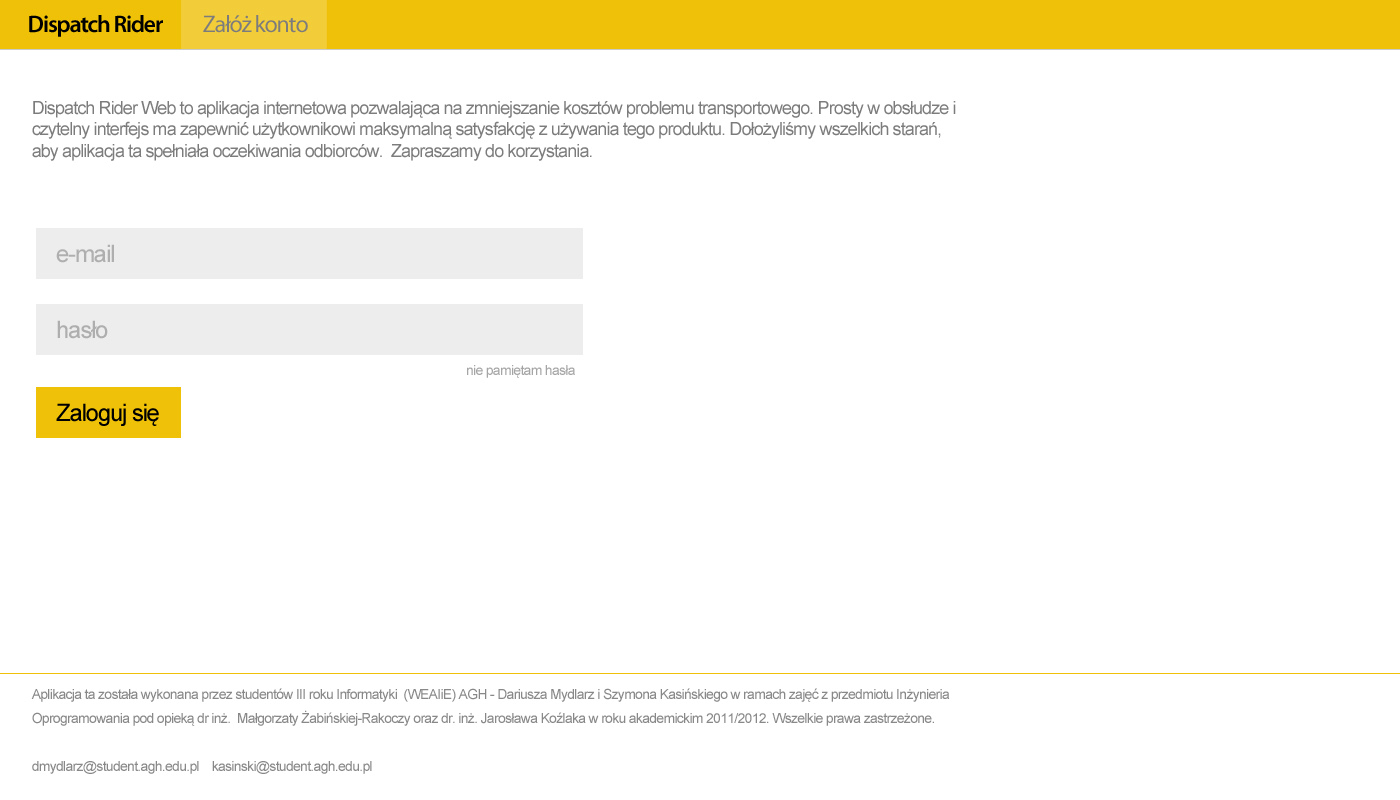
\includegraphics[scale=0.3]{imgs/unlogged_home.jpg}
\caption{Strony powitalna}
\label{fig:home_page}
\end{figure}
\end{center}

\vfill\hfill

\begin{center}
\begin{figure}[H]
\centering
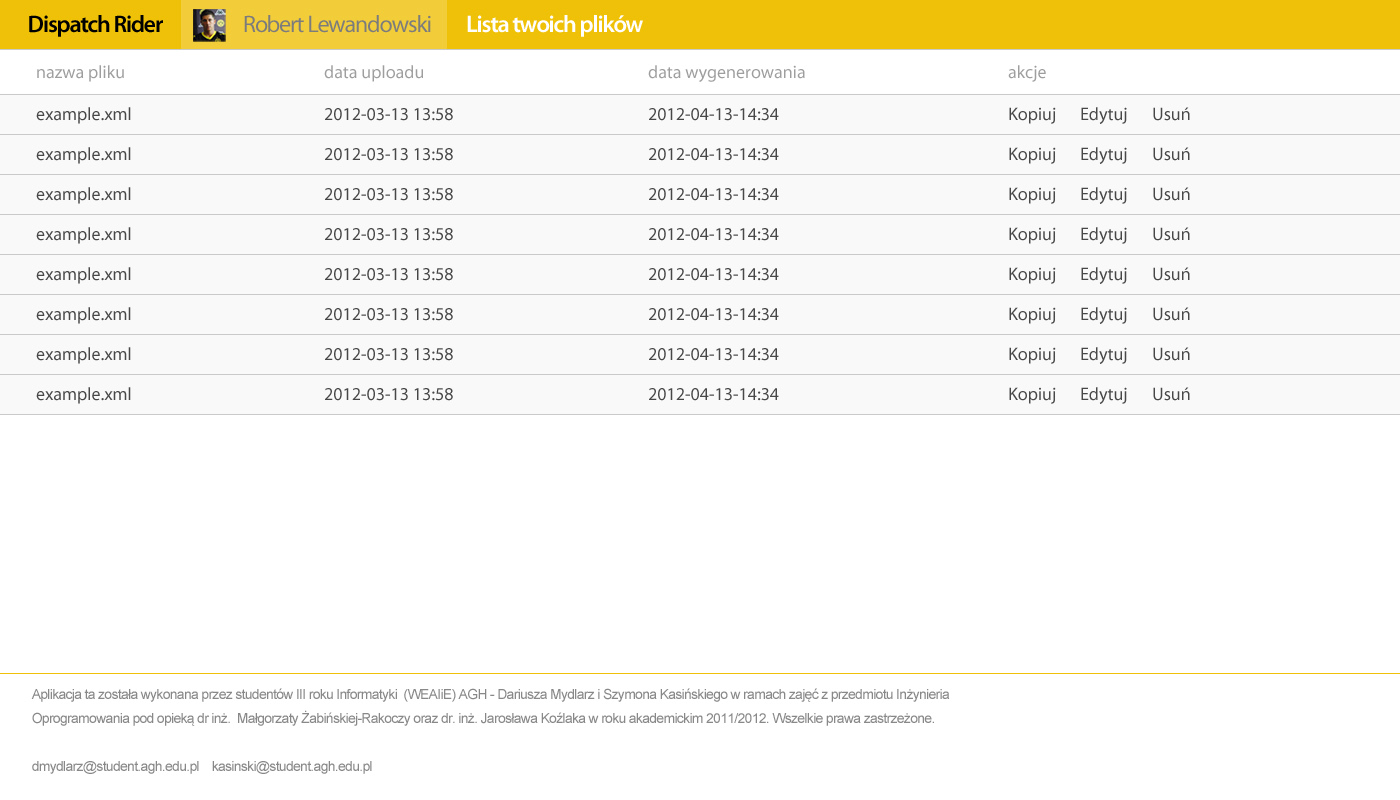
\includegraphics[scale=0.3]{imgs/logged_home.jpg}
\caption{Lista zadań}
\label{fig:tasks_list}
\end{figure}
\end{center}

\begin{center}
\begin{figure}[H]
\centering
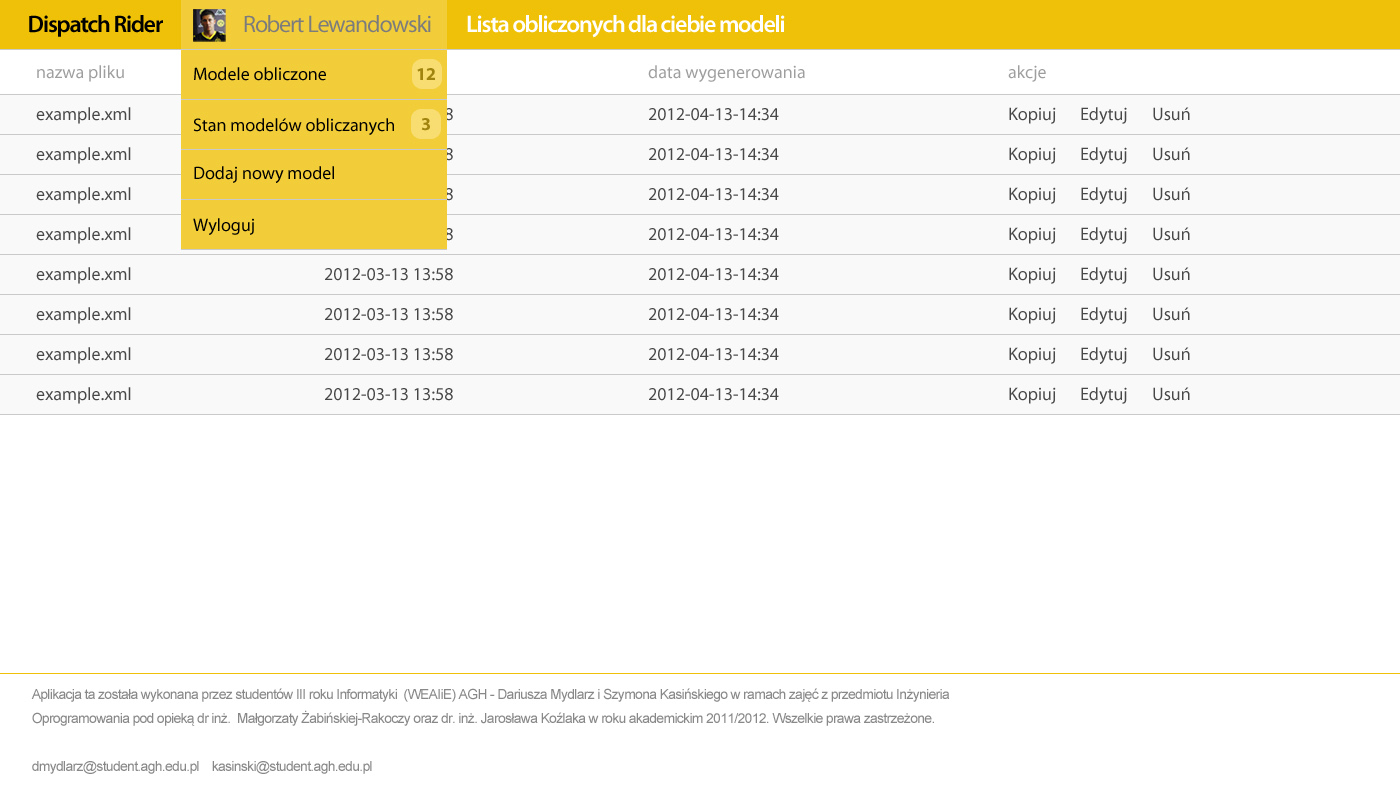
\includegraphics[scale=0.3]{imgs/logged_home_menu.jpg}
\caption{Menu aplikacji}
\label{fig:app_menu}
\end{figure}
\end{center}

\begin{center}
\begin{figure}[H]
\centering
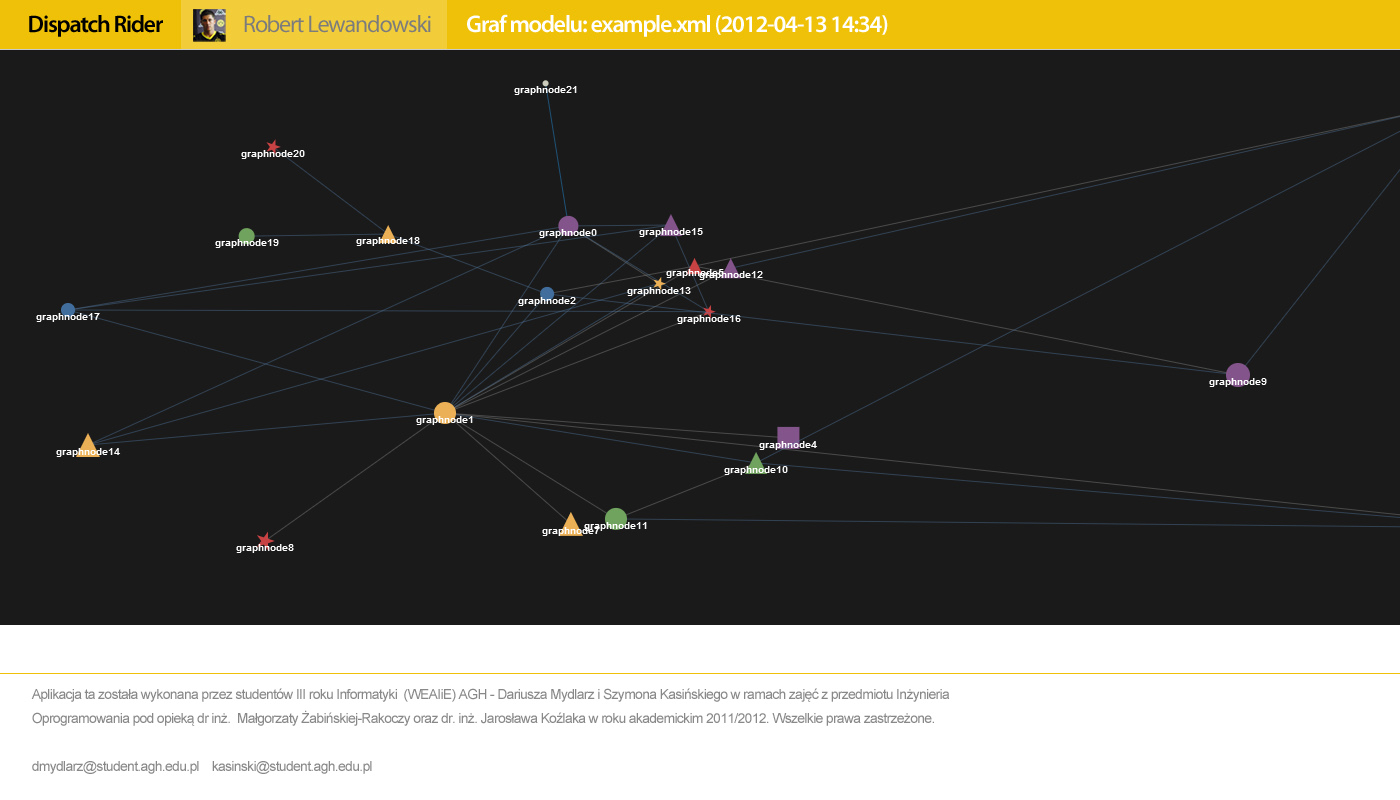
\includegraphics[scale=0.3]{imgs/logged_graph_viewjpg.jpg}
\caption{Widok grafu}
\label{fig:graph_view}
\end{figure}
\end{center}
